O momento aplicado é dado pela equação:

\begin{equation}
  M = \frac{P}{n} \cdot 955 \cdot K
  \label{eq:momento_aplicado}
\end{equation}

Onde:

\begin{itemize}[leftmargin=1.25cm]
  \item $M$: momento aplicado em $\si{\deca\newton\meter}$.
  \item $P$: potência do redutor em $\si{\kilo\watt}$ (Tabela \ref{tab:dados_redutor_adotado}).
  \item $n$: rotação de saída em $\si{\rpm}$ (Tabela \ref{tab:dados_redutor_adotado}).
  \item $K$: fator de serviço.
\end{itemize}

\vspace{1em}

Considerou-se um fator de serviço $K = \num{1.25}$ com base na tabela do catálogo de acoplamentos da Gosan para o grupo do mecanismo $1AM$.

\begin{figure}[H]
  \centering
  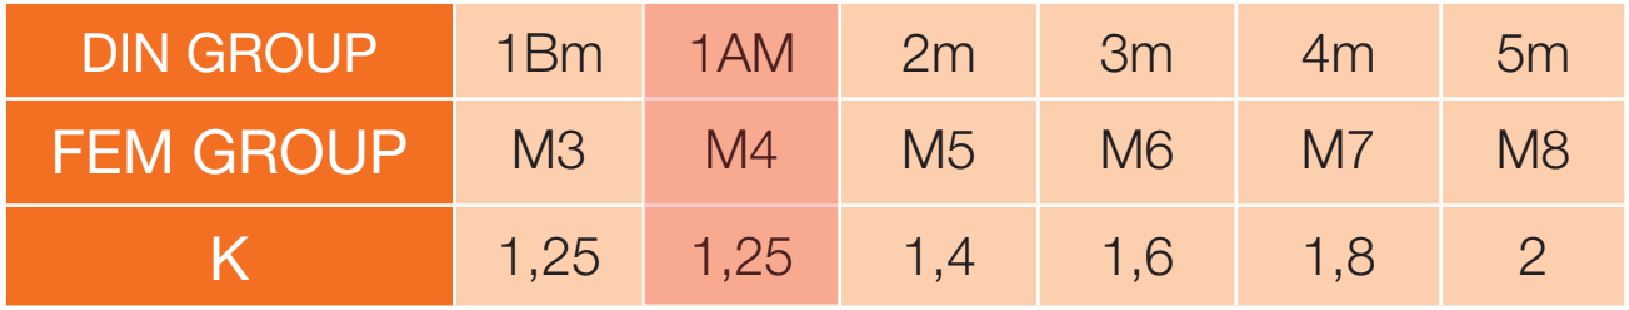
\includegraphics[width=0.6\textwidth]{content/sections/03_sistema_de_elevacao/sections/03_conjunto_do_acionamento_do_sistema_de_elevacao/sections/06_acoplamento_redutor_tambor/figures/k_gosan.pdf}
  \caption{Fator de serviço para o acoplamento \cite[p.~3]{gosan_acoplamentos}}
  \label{fig:k_gosan}
\end{figure}

Substituindo os valores na equação \eqref{eq:momento_aplicado}:

\begin{align*}
  M & = \frac{32}{10} \cdot 955 \cdot \num{1.25} \\
  M & = \boxed{\SI{3820}{\deca\newton\meter}}
\end{align*}

Com base no catálogo de acoplamentos rígidos da Gosan, selecionou-se um acoplamento rígido com torque máximo de $\SI{4050}{\deca\newton\meter}$. As figuras e a tabela a seguir apresentam os dados extraídos do catálogo para o acoplamento adotado:

\begin{figure}[H]
  \centering
  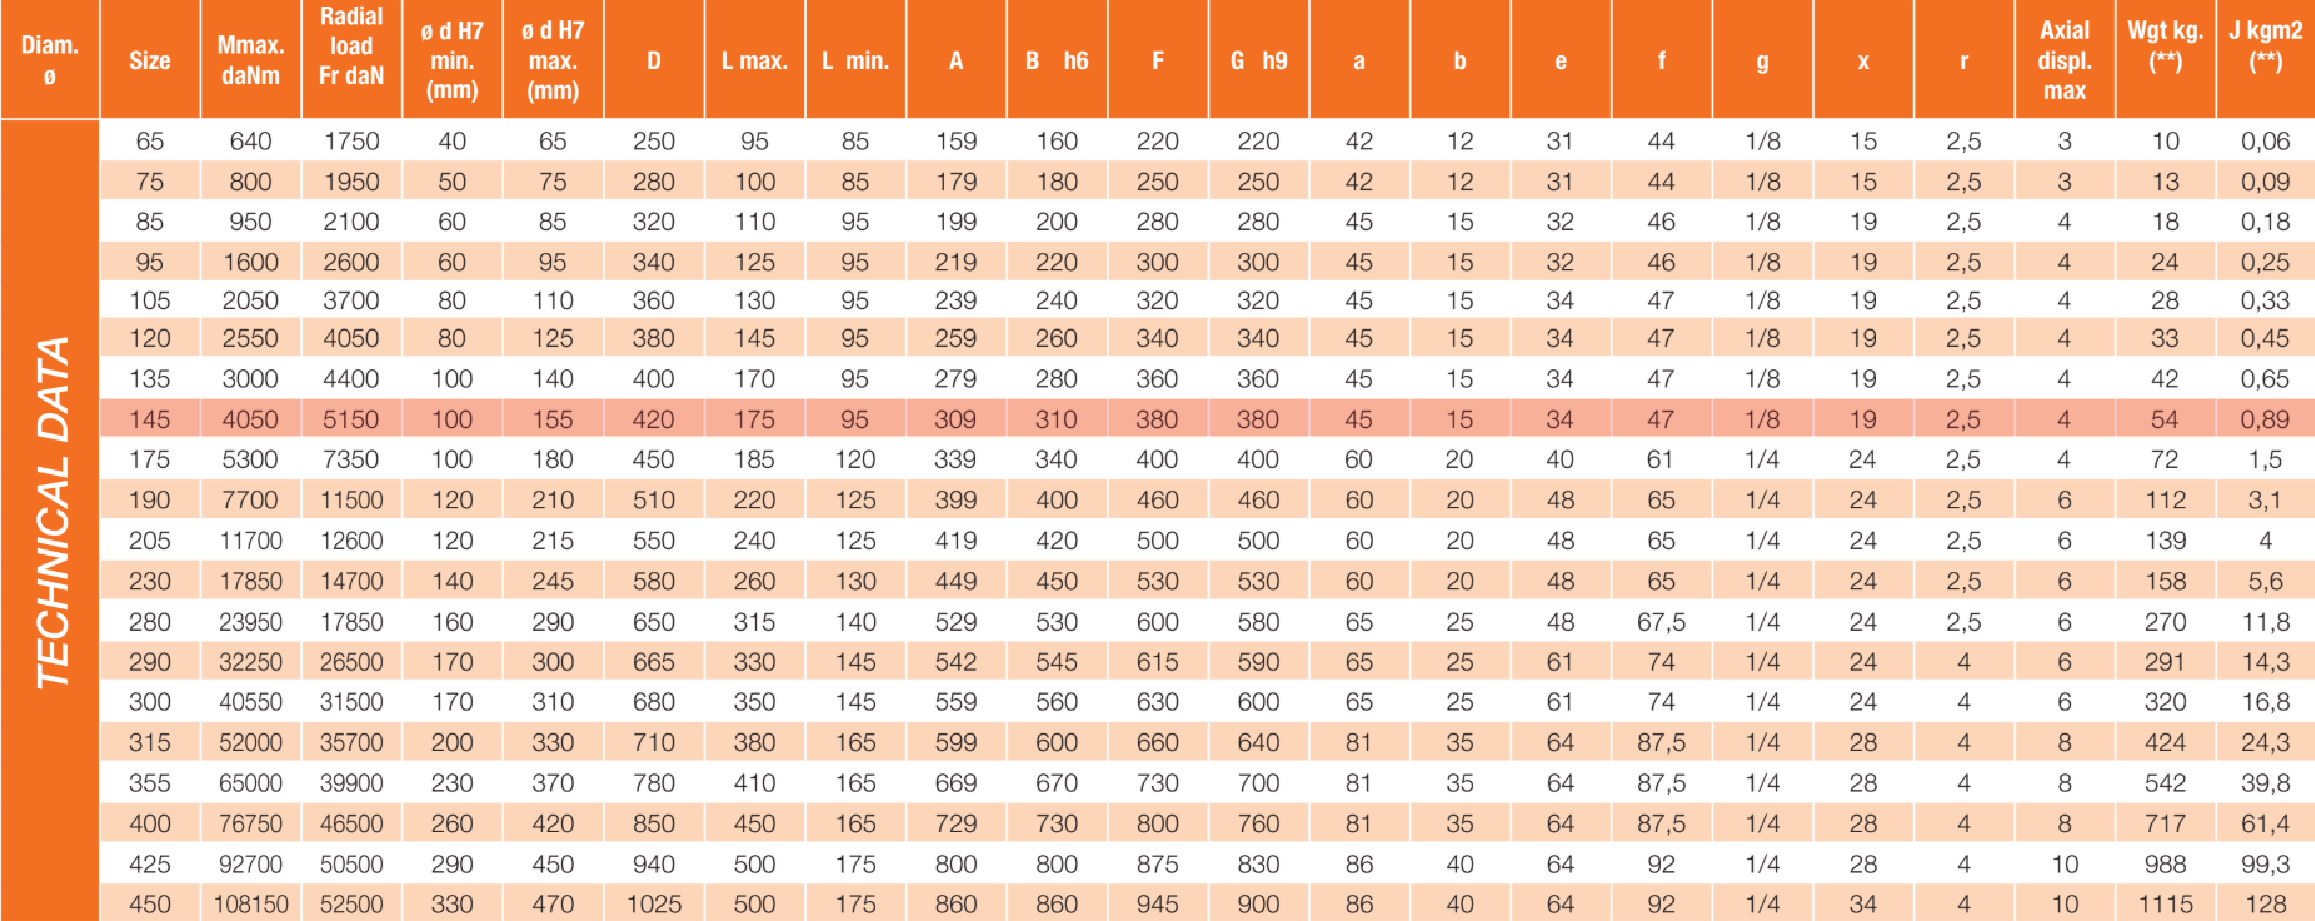
\includegraphics[width=1\textwidth]{content/sections/03_sistema_de_elevacao/sections/03_conjunto_do_acionamento_do_sistema_de_elevacao/sections/06_acoplamento_redutor_tambor/figures/catalogo_gosan.pdf}
  \caption{Catálogo de acoplamentos rígidos \cite[p.~4]{gosan_acoplamentos}}
  \label{fig:catalogo_gosan}
\end{figure}

\begin{figure}[H]
  \centering
  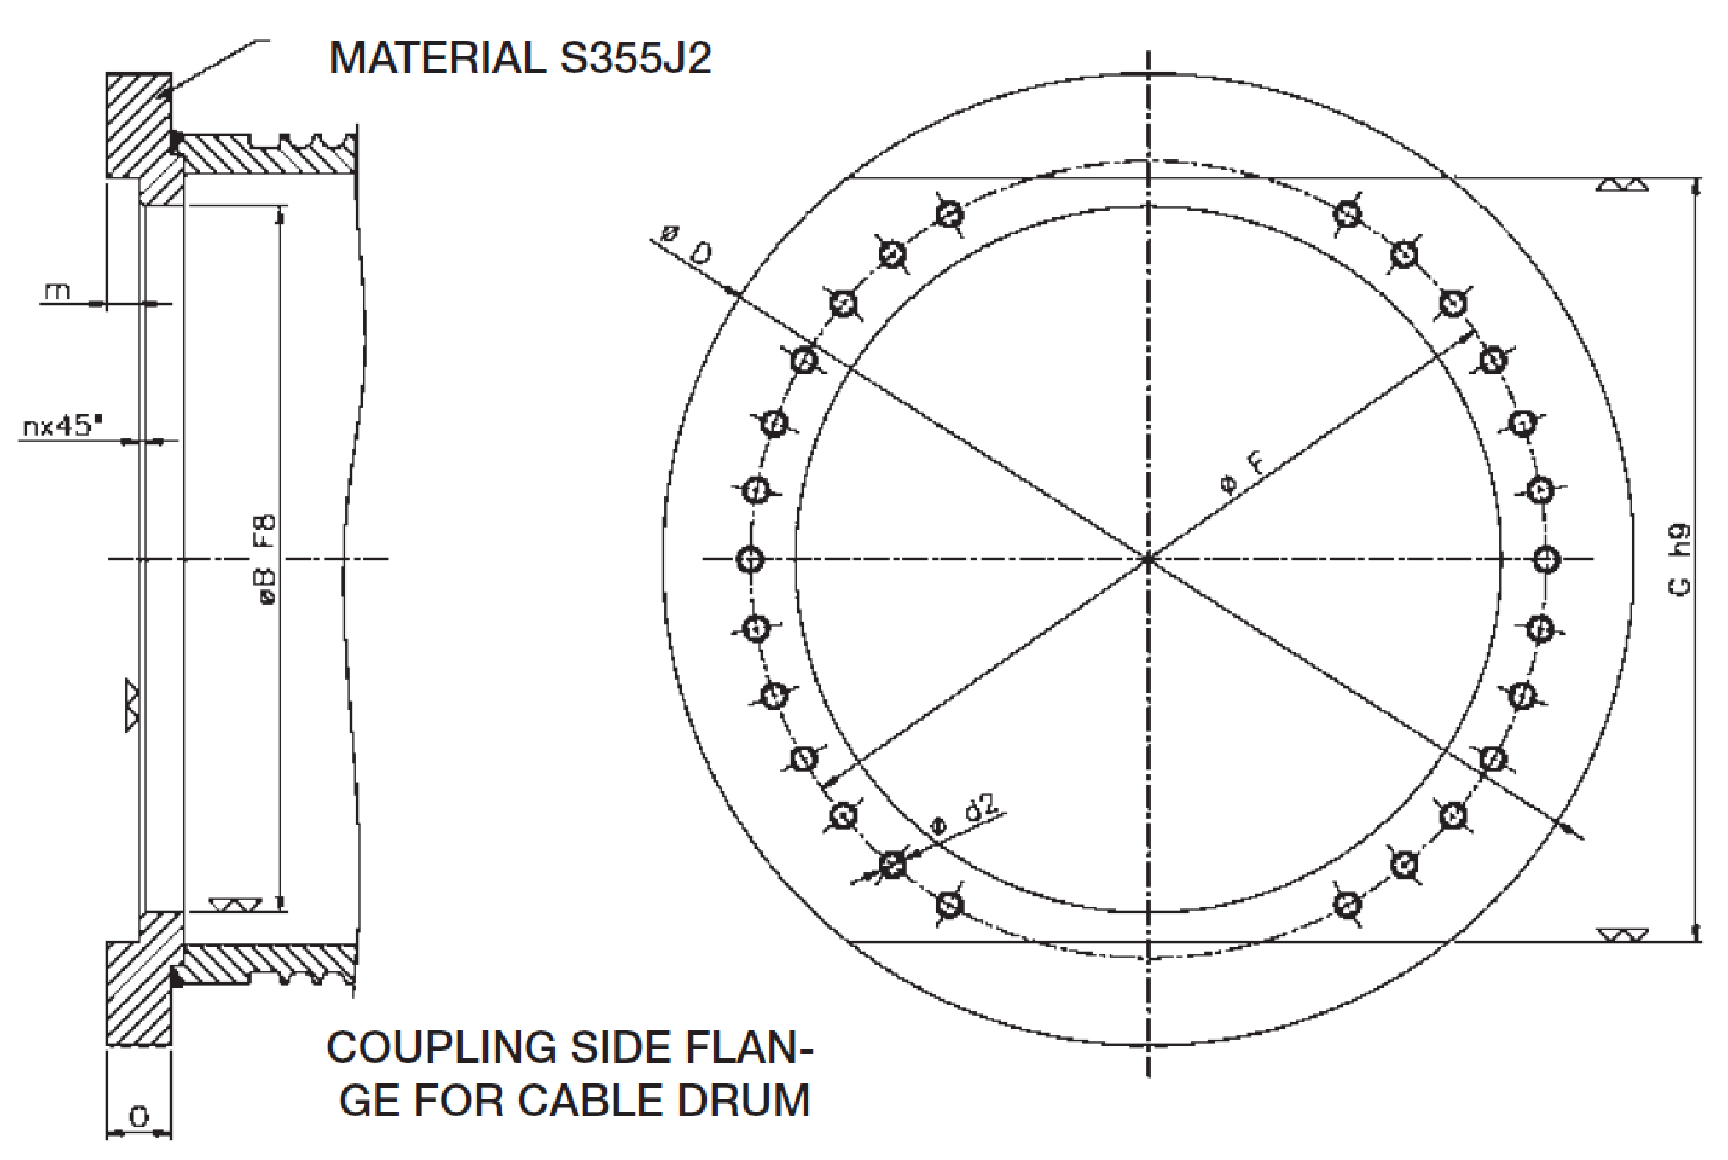
\includegraphics[width=1\textwidth]{content/sections/03_sistema_de_elevacao/sections/03_conjunto_do_acionamento_do_sistema_de_elevacao/sections/06_acoplamento_redutor_tambor/figures/flange_gosan.pdf}
  \caption{Desenho do flange de fixação do tambor \cite[p.~4]{gosan_acoplamentos}}
  \label{fig:flange_gosan}
\end{figure}

\begin{figure}[H]
  \centering
  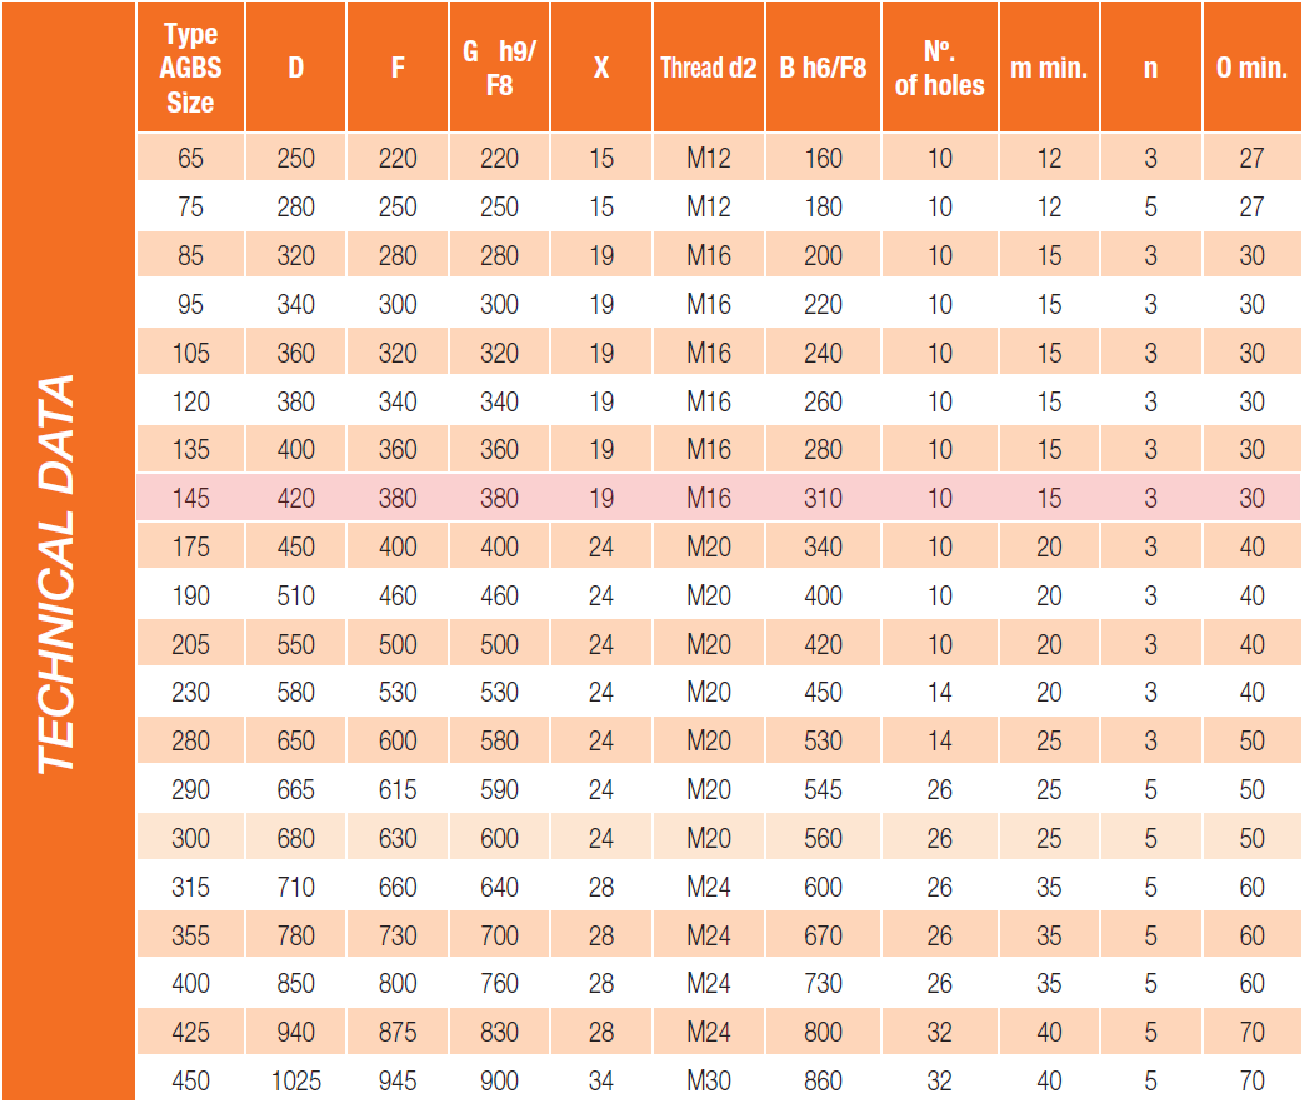
\includegraphics[width=0.7\textwidth]{content/sections/03_sistema_de_elevacao/sections/03_conjunto_do_acionamento_do_sistema_de_elevacao/sections/06_acoplamento_redutor_tambor/figures/dim_flange_gosan.pdf}
  \caption{Dimensões do flange de fixação do tambor \cite[p.~4]{gosan_acoplamentos}}
  \label{fig:dim_flange_gosan}
\end{figure}

\begin{table}[H]
  \centering
  \caption{Dados do acoplamento adotado segundo o catálogo da Gosan}
  \label{tab:dados_acoplamento_tambor}
  \begin{tabularx}{\textwidth}{>{\centering\arraybackslash}X>{\centering\arraybackslash}X>{\centering\arraybackslash}X}
    \toprule
    Descrição                      & Símbolo          & Valor                         \\
    \midrule
    Diâmetro mínimo do eixo        & $d_{\text{min}}$ & \SI{100}{\milli\meter}        \\
    Diâmetro máximo do eixo        & $d_{\text{max}}$ & \SI{155}{\milli\meter}        \\
    Momento máximo                 & $M_{\text{max}}$ & \SI{4050}{\deca\newton\meter} \\
    Carga radial                   & $F_r$            & \SI{5150}{\deca\newton}       \\
    Diâmetro externo para o flange & $D$              & \SI{420}{\milli\meter}        \\
    Espessura mínima do flange     & $e_f$            & \SI{30}{\milli\meter}         \\
    Massa                          & $m$              & \SI{54}{\kilogram}            \\
    \bottomrule
  \end{tabularx}
\end{table}

O tambor adotado possui um diâmetro interno de $\SI{307.94}{\milli\meter}$, que está próximo ao diâmetro interno definido no catálogo de $\SI{310}{\milli\meter}$.
